%%%%%%%%%%%%%%%%%%%%%%%%%%%%%%%%%%%%%%%%%
% Large Colored Title Article
% LaTeX Template
% Version 1.1 (25/11/12)
%
% This template has been downloaded from:
% http://www.LaTeXTemplates.com
%
% Original author:
% Frits Wenneker (http://www.howtotex.com)
%
% License:
% CC BY-NC-SA 3.0 (http://creativecommons.org/licenses/by-nc-sa/3.0/)
%
%%%%%%%%%%%%%%%%%%%%%%%%%%%%%%%%%%%%%%%%%

%----------------------------------------------------------------------------------------
%	PACKAGES AND OTHER DOCUMENT CONFIGURATIONS
%----------------------------------------------------------------------------------------

\documentclass[DIV=calc, paper=a4, fontsize=11pt, twocolumn]{scrartcl}	 % A4 paper and 11pt font size

\usepackage{lipsum} % Used for inserting dummy 'Lorem ipsum' text into the template
\usepackage[english]{babel} % English language/hyphenation
\usepackage[protrusion=true,expansion=true]{microtype} % Better typography
\usepackage{amsmath,amsfonts,amsthm} % Math packages
\usepackage[svgnames]{xcolor} % Enabling colors by their 'svgnames'
\usepackage[hang, small,labelfont=bf,up,textfont=it,up]{caption} % Custom captions under/above floats in tables or figures
\usepackage{booktabs} % Horizontal rules in tables
\usepackage{fix-cm}	 % Custom font sizes - used for the initial letter in the document
\usepackage{graphicx}
\usepackage{hyperref}
\usepackage{cleveref}

 
\usepackage{sectsty} % Enables custom section titles
\allsectionsfont{\usefont{OT1}{phv}{b}{n}} % Change the font of all section commands

\usepackage{fancyhdr} % Needed to define custom headers/footers
\pagestyle{fancy} % Enables the custom headers/footers
\usepackage{lastpage} % Used to determine the number of pages in the document (for "Page X of Total")

% Headers - all currently empty
\lhead{}
\chead{}
\rhead{}

% Footers
\lfoot{}
\cfoot{}
\rfoot{\footnotesize Page \thepage\ of \pageref{LastPage}} % "Page 1 of 2"

\renewcommand{\headrulewidth}{0.0pt} % No header rule
\renewcommand{\footrulewidth}{0.4pt} % Thin footer rule

\usepackage{lettrine} % Package to accentuate the first letter of the text
\newcommand{\initial}[1]{ % Defines the command and style for the first letter
\lettrine[lines=3,lhang=0.3,nindent=0em]{
\color{DarkGoldenrod}
{\textsf{#1}}}{}}

%----------------------------------------------------------------------------------------
%	TITLE SECTION
%----------------------------------------------------------------------------------------

\usepackage{titling} % Allows custom title configuration

\newcommand{\HorRule}{\color{DarkGoldenrod} \rule{\linewidth}{1pt}} % Defines the gold horizontal rule around the title

\pretitle{\vspace{-30pt} \begin{flushleft} \HorRule \fontsize{40}{40} \usefont{OT1}{phv}{b}{n} \color{DarkRed} \selectfont} % Horizontal rule before the title

\title{Will Living People Ever Outnumber the Dead?} % Your article title


\posttitle{\par\end{flushleft}\vskip 0.5em} % Whitespace under the title

\preauthor{\begin{flushleft}\large \lineskip 0.5em \usefont{OT1}{phv}{b}{sl} \color{DarkRed}} % Author font configuration

\author{\href{http://www.physics.wustl.edu/smirshekari}{Saeed Mirshekari} \thanks{smirshekari@ift.unesp.br} \thanks{Thanks to M.~Le Delliou for useful discussions.
}\; } % Your name
\postauthor{\footnotesize \usefont{OT1}{phv}{m}{sl} \color{Black} % Configuration for the institution name
%Ph.D. in Physics, %Sao P\~{a}ulo, Brazil % Your institution
%smirshekari@wustl.edu %  Your email address
%\today
28 February, 2014

\par\end{flushleft}\HorRule} % Horizontal rule after the title
\date{} % Add a date here if you would like one to appear underneath the title block


%----------------------------------------------------------------------------------------

\begin{document}

\maketitle % Print the title

\thispagestyle{fancy} % Enabling the custom headers/footers for the first page 

%----------------------------------------------------------------------------------------
%	ABSTRACT
%----------------------------------------------------------------------------------------

% The first character should be within \initial{}
\initial{P}\textbf{robably not! It has been shown that only about 6.5 percent of all people ever born were alive in 2011~\cite{Carl}. But the human population on Earth has been growing very rapidly in the recent decades such that one could imagine one day in which the number of alive people reaches the number of all the dead people. Assuming the world's average life expectancy to remain constant and equal to its current value ($68$ years) and the world's annual growth rate to stay constant but just a bit less than its current value ($1\%$), we show that living people will never outnumber the dead.\footnote{This calculations might be vey well know and we probably just have rediscoved them one more time.}}

%----------------------------------------------------------------------------------------
%	ARTICLE CONTENTS
%----------------------------------------------------------------------------------------

%%%%%%%%%%%%%%%%%%%%%%%%
\section*{Growth of Living Population}
The human population has started to grow extremely fast only since the last few centuries, as you can see in Figure~\ref{fig:popcurve}. The rate of population growth has obviously changed over time. But, because of all the human improvements and developments in the modern world it is not unlikely to reach a constant rate of population growth and life expetancy in the future.

\begin{figure}
\centering
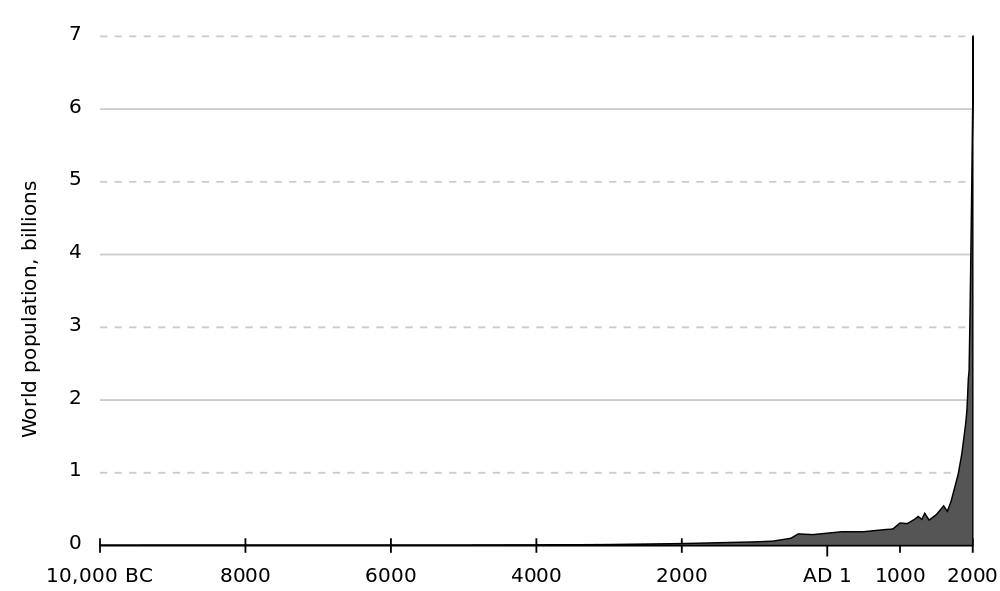
\includegraphics[width=9cm]{Population_curve.png}
\caption{The estimated size of human population from 10,000 BCE--2000 CE. \cite{wikipedia}}
\label{fig:popcurve}
\end{figure}

The ``annual population growth rate'' ($r$) is the rate at which the number of individuals in a population increases in a year as a fraction of the initial population. It is very easy to show that for a constant population rate of $r$ the living population will be growing as 

\begin{equation}
\text{Alive}(t) = N_0 (1+r)^t,
\label{alive}
\end{equation}
where $N_0$ is the living population at the initial time. Population in the world is currently growing at a rate of  about $1.14\%$ per year~\cite{worldometers} and the current world's average life expectancy is $67.88$ years~\cite{wikipedia}. 

%%%%%%%%%%%%%%%%%%%%%%%%
\section*{How Many People Are Dead?}
Knowing only the constant values of current annual population growth rate, $r$, and the world average life expectancy, $\langle L\rangle$, there is a simple way to estimate the number of dead people at time $t$. 

Suppose after $t=t_0$ the annual growth rate and the average life expectancy reach their constant values. The number of living people at this time is given by Equation~(\ref{alive}) as Alive$(t_0)$. Now the question is that after a single period of the average life expectancy, i.e. at $t=t_0+\langle L\rangle$, how many people have died in average in this time period? The answer is simply Alive$(t_0)$. In other words, in average, the number of people who have died since $t=t_0$ until $t=t_0+\langle L\rangle$ is same as the number of people who were alive at $t=t_0$. Without losing any generality we can set $t_0=0$ and generalize this idea to the future times in which $t^*=N \langle L\rangle$ and write
\begin{equation}
\text{Dead}(t^*) = \sum_{n=0}^{N-1} \text{Alive}(n \langle L\rangle)+ \text{Dead}(t_0) 
\end{equation}
where $N$ is an integer number and $\text{Dead}(t_0)$ is the number of all people who have died at any time in the history before $t=t_0$. Using Equation~(\ref{alive}), the above summation can get as simplified as
\begin{equation}
\text{Dead}(t) = N_0 \frac{(1+r)^{t}-1}{(1+r)^{\langle L\rangle}-1} + \text{Dead}(t_0).
\label{dead}
\end{equation}


%%%%%%%%%%%%%%%%%%%%%%%%
\section*{Critical Values of $r$ and $\langle L\rangle$}
Based on Equations (\ref{alive}), (\ref{dead}), it's not difficult to show the living population ultimately outnumber the dead if and only if:
\begin{equation}
(1+r)^{\langle L\rangle} > 2.
\end{equation}
For example, with the current value of the world average life expectancy, i.e. $67.88$ years, the living population can outnumber the dead if and only if the annual population growth rate is not less than the critical value of $1.02\%$. This number is only slightly smaller than the current value for the world i.e. $1.14\%$. Although we have considered $r$ to be constant, recent studies~\cite{worldometers} predict a small decrease in the rate of population growth to a value less than $1\%$ in close future. This small decrease would be enough to conclude that the living population never outnumber the dead with the current world average value of life expectancy.

On the other hand, as another example, if we fix the population growth rate at its current value, the world average life expectancy has to be greater than $61.12$ years to ultimately allow the living population outnumber the dead. Any values of $r$ and $\langle L\rangle$ less than their critical values cause the dead population outnumber the living forever.

%----------------------------------------------------------------------------------------
%	Acknowledgement
%----------------------------------------------------------------------------------------
%\section*{Acknowledgements}
%----------------------------------------------------------------------------------------
%	REFERENCE LIST
%----------------------------------------------------------------------------------------

\begin{thebibliography}{99} % Bibliography - this is intentionally simple in this template

\bibitem{Carl} Carl Haub, \href{http://www.prb.org/Publications/Articles/2002/HowManyPeopleHaveEverLivedonEarth.aspx}{http://www.prb.org} (2011)
\bibitem{worldometers} http://www.worldometers.info
\bibitem{wikipedia} http://www.wikipedia.org

\end{thebibliography}

%----------------------------------------------------------------------------------------

\end{document}